\documentclass[12pt]{article}
\usepackage[utf8]{inputenc}
\usepackage[round]{natbib}
\usepackage{amsmath}
\usepackage{amssymb}
\bibliographystyle{plainnat}
\usepackage[top=0.6in, bottom=0.6in, left=0.7in, right=0.7in]{geometry}
\usepackage{graphicx}
\usepackage{float}
\usepackage{hyperref}
\usepackage{algorithm, algorithmic}

\graphicspath{{images/}}
\newcommand{\argmin}{\mathop{\mathrm{argmin}}}
\newcommand{\pbreak}{\vspace{4mm}}

\title{\rule{\linewidth}{2pt}\\\vspace{2mm}
Can random choices alleviate the burden of hyper-parameter optimization and model selection for neural networks?\\
\rule{\linewidth}{2pt}}
\author{Vishwak Srinivasan\\\texttt{cs15btech11043}
\and
Harsh Agarwal\\\texttt{cs15btech11019}}
\date{}

\begin{document}
\maketitle

\section{Introduction}
\begin{flushleft}
A critical step in hyper-parameter optimization and model selection in neural networks is to make a set of choices. These choices could be the learning rate, number of layers in a neural network, number of nodes in each layer of the neural network, weight decay parameters and so on. If we were to denote these set of choices by \(\Lambda\), then the goal of hyper-parameter optimization and model selection is to find the ideal \(\lambda^{*} \in \Lambda\) such that given a hyper-parameter objective \(\Psi\) (which could be cross-validation loss),
\begin{equation}
\lambda^{*} = \argmin_{\lambda \in \Lambda} \Psi(\lambda)
\end{equation}

Generally, if provided with \(K\) such configurable parameters, then \(\Lambda\) would be a set of \(K\)-tuples. Let the set of ``valid'' choices for each of the \(K\) configurable (hyper)parameters be \(C_{i}\), \(\forall i \in \{1, \ldots, K\}\). Now, the space of valid parameter combinations is \(\displaystyle \prod_{i=1}^{K} C_{i}\), which is affected by the curse of dimensionality.
\pbreak

There have been multiple attempts at improving hyperparameter optimization over the years. The most commonly used method is \textbf{grid search}, which is embarrasingly parallel, and hence can be done ``efficiently''. However, the task of determining the sets \(\displaystyle \lbrace C_{i} \rbrace_{i=1}^{K}\) remains, for which \textbf{manual search} is used, where one can identify regions in \(\Lambda\) that are more productive and promising, and these regions can be used to build the sets \(\displaystyle \lbrace C_{i} \rbrace_{i=1}^{K}\). Recently \citet{random-search} have provided an algorithm for hyper-parameter optimization called \textbf{random search}, which suggests that a search based entirely on random events is capable of finding, over the same domain \(\Lambda\), hyper-parameters and models which are just as good or even better than the ones found by grid search, with a fraction of the computation time and consequently energy.
\end{flushleft}

\section{Previous Work and Our Contributions}
\subsection{Previous Work}
\begin{flushleft}
In addition to \textbf{grid / manual search} and \textbf{random search} specified above, there have been multiple efforts aimed at speeding up hyper-parameter optimization. \citet{bayesian-hyp-opt} present a Bayesian approach to hyper-parameter with certain theoretical guarantees, and evaluate their method for model selection for object recognition tasks. \citet{grad-hyp-opt} compute hyper-parameter gradients by exactly reversing the dynamics of stochastic gradient descent with momentum. A bandit approach towards hyper-parameter optimization was also proposed in \citet{bandit-hyp-opt}.
\pbreak

The idea of having an ensemble of neural networks dates back to 1990 stemming from the work of \citet{tpami-ensemble-1990}. A few years later, work by \citet{nips-ensemble-1995} also suggested the usage of neural network ensemble for improved generalization. However, a major drawback of these prior studies focus on improving the generalization performance, while few of them address the cost of training ensembles.
\pbreak

\citet{nc-ensemble-2000} performed another empirical study where they propose three methods to couple AdaBoost and neural classifiers. The authors state in their paper that one method gave good generalization, but however required more training epochs and the second-order batch method such as conjugate gradients.
\pbreak

A very recent study conducted by \citet{arxiv-ensemble-2017} showed that a variant called the ``Super-Learner'' gave a performance boost among many other variants in their work, with an accuracy bump of 1\% on the CIFAR10 dataset.
\end{flushleft}

\subsection{Our Contributions}
\begin{flushleft}
As the title may suggest, the goal of the project was to develop / build random neural network models and see if an ensemble of these ``random'' models would perform just as well or better than those models found after an extensive hyper-parameter search by either one of the methods specified above minus the time.
\pbreak

Running grid search for other model hyper-parameters for a neural network with 3 hidden layers took a lot of time, meaning a direct comparison would not be possible. As a solution to this issue, our first contribution was the implementation of \textbf{random search} over the set of model parameters.
\pbreak

Now that a baseline has been achieved, the next contribution of the work is the implementation of an ensemble of neural networks. The ensemble built was a simple weighted hard-soft voting classifier. Using this, we will be checking the hypothesis posed empirically.
\end{flushleft}

\section{Contribution 1: Random Search over\\ model Hyper-parameters}
\begin{flushleft}
The model hyper-parameters considered for performing a search over are listed below:
\begin{itemize}

\item Model Shape and Shape Parameters: We assume shapes for a given neural network: \texttt{decreasing}, \texttt{convex}, \texttt{concave} and \texttt{constant}. Associated with these ``shapes'' are two parameters. Examples of neural networks constructed with these shapes are shown in Figure \ref{shapes}.
\begin{figure}[ht]
\begin{minipage}{0.24\linewidth}
\centering
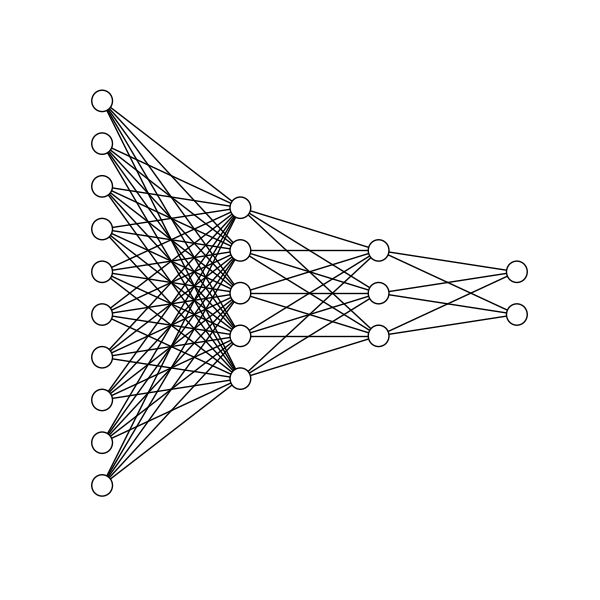
\includegraphics[width=0.95\textwidth]{decreasing-eg.png}
\end{minipage}
\begin{minipage}{0.24\linewidth}
\centering
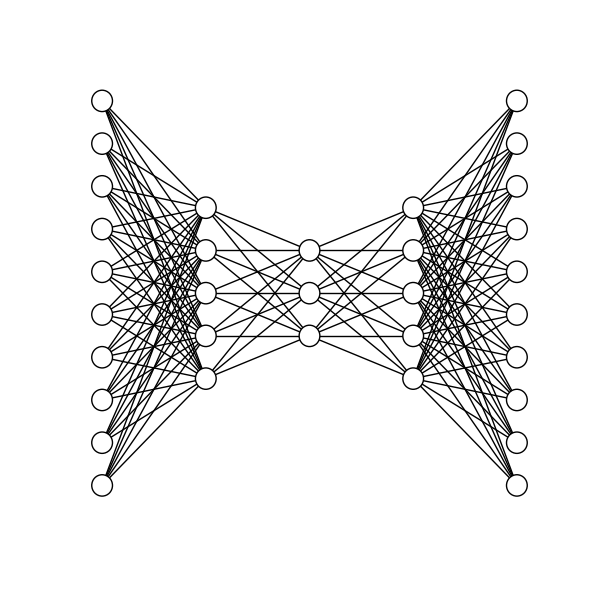
\includegraphics[width=0.95\textwidth]{convex-eg.png}
\end{minipage}
\begin{minipage}{0.24\linewidth}
\centering
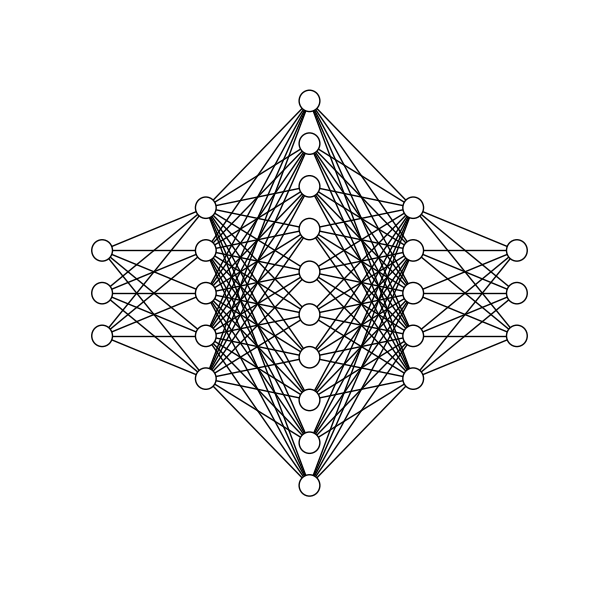
\includegraphics[width=0.95\textwidth]{concave-eg.png}
\end{minipage}
\begin{minipage}{0.24\linewidth}
\centering
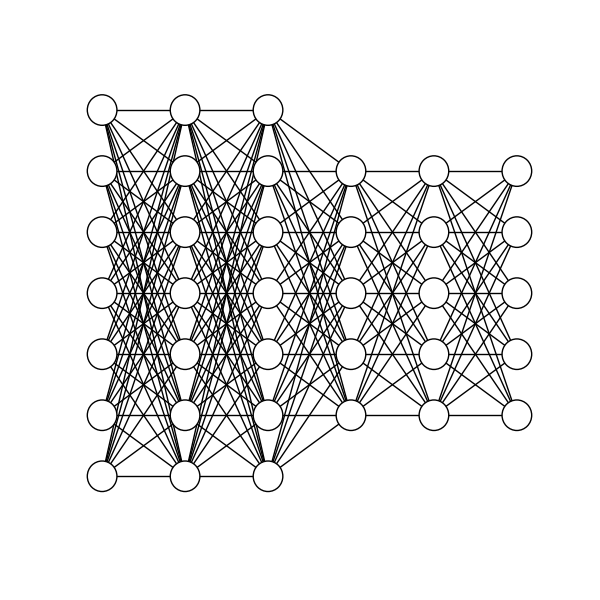
\includegraphics[width=0.95\textwidth]{constant-eg.png}
\end{minipage}
\caption{(L to R): \texttt{decreasing}, \texttt{convex}, \texttt{concave} and \texttt{constant} shapes respectively}
\label{shapes}
\end{figure}

\item Number of Hidden layers: Number of hidden layers between the input and output layers
\item Dropout probabilities: Layer-wise dropout probability, where \texttt{Dropout(p)}, denotes that Dropout with probability \(p\) (\citet{dropout}). 
\item Existence of batch normalization: Layer-wise boolean vector representing the existence of batch normalization for that layer. Note that since we are using MLPs, a 1-D version of the Batch Normalization(\citet{batchnorm}) is used.
\item Weight Initialization technique: Considering the fact that weight initialization plays a crucial role in the performance of the neural network, we have decided to include this in the set of model hyper-parameters. The implemented initialization schemes are Glorot's initializaton\cite{glorot}, Kaiming He's initialization\cite{he}, a \(\mathcal{U}[0, 1]\) initialization and the default initialization i.e., \(\sqrt{\frac{1}{\text{fan-out}}}\)
\item Activation functions: One-activation-per-network is used, to reduce the dimensionality of the search space. The activations are \texttt{ReLU}, \texttt{sigmoid} and \texttt{tanh}.
\end{itemize}

Initially, we attempted at running grid search over a discretized search space (where the continuous variables were discretized) resulting in \(\approx 7000\) grid points with the negative log likelihood loss over the validation set as a scoring function. The neural networks built on this grid were made to train for 3 epochs on every dataset. Despite using 3 GPUs\footnote{NVIDIA 1080Ti} for 2 days, the experiments failed to complete, causing us to time-out the experiments in the interest of freeing resources. The power during this period was 80W per GPU (on average), thus equating to 240W overall (on average)\footnote{Power values where obtained using \texttt{nvidia-smi}}.
\pbreak

Going with the random search algorithm, we consider 1000 samples drawn with replacement while maintaining the same scoring function as specified above. This took relatively less time to finish (\(\approx\) 7 hrs) on 1 GPU. After obtaining these results, we finetuned the architecture to get our best results. Below tabulated are those results. These results are averaged over 5 runs. \texttt{BN} indicates a Batch Normalization layer, and \texttt{DP(p=p)} indicates a Dropout layer with probability \(p\).
\begin{center}
\begin{tabular}{|c|c|p{0.65\linewidth}|}
\hline
\textbf{Dataset} & \textbf{Accuracy} & \textbf{Architecture}\\
\hline
\hline
MNIST & \(98.294 \pm 0.112\)\% & 784 - 1097 - \texttt{ReLU} - 329 - \texttt{BN} - \texttt{ReLU} - 98 - \texttt{BN} - \texttt{ReLU} - 10 - \texttt{Softmax}\\
\hline
CIFAR10 & \(95.018 \pm 0.021\)\% & 256 - 153 - \texttt{ReLU} - 99 - \texttt{ReLU} - \texttt{DP(p=0.25)} - 64 - \texttt{ReLU} - \texttt{DP(p=0.5)} - 10 - \texttt{Softmax}\\
\hline
SVHN & \(96.262 \pm 0.027\)\% & 192 - 96 - \texttt{ReLU} - \texttt{DP(p=0.25)} - 124 - \texttt{ReLU} - \texttt{DP(p=0.25)} - 161 - \texttt{ReLU} - \texttt{DP(p=0.5)} - 10 - \texttt{Softmax}\\
\hline
\end{tabular}
\end{center}

All these networks were initialized using Glorot's initialization technique.
\end{flushleft}

\section{Contribution 2 - Ensembles}
\begin{flushleft}
The main motivation for the usage of ensembles is mostly due to the time it takes for performing a search. Computation costs still remain the bottleneck of such methods, and hence why not train multiple random architectures and treat them as an ensemble instead of wasting valuable compute time, albeit some additional memory expenditure?
\pbreak

Our random networks are experimented with ensembles of size 3, 4 and 5 i.e., the number of random neural networks. These random neural networks are generated by randomizing all the hyper-parameters stated above. The ensemble under consideration is a simple voting ensemble. This voting ensemble allows for parallelization of training of candidate networks. The voting ensemble also takes in a set of weights representing the amount of confidence of judgement of each neural network. These weights are assigned based of network features:
\begin{itemize}
\item Uniform
\item Number of hidden layers
\item Number of Dropout layers
\item Number of Batch Normalization layers
\end{itemize}

Additionally, the ensemble can also choose to take a hard decision or a soft decision. A soft decision is based on the weighted average of class probabilities, and a hard decision is based on the maximum weight for a class.
\pbreak

We evaluated this ensemble on the same datasets above, and the results are tabulated below. These results were averaged over 5 trials.
\begin{center}
\begin{tabular}{|c|c|c|c|c|}
\hline
\textbf{Dataset} & \textbf{\# networks} & \textbf{Voting type} & \textbf{Weighing scheme} & \textbf{Accuracy} \\
\hline
\hline
MNIST & 3 & Soft & Number of Hidden Layers & 97.74\% \\
\hline
CIFAR10 & 3 & Hard & Uniform & 95.04\% \\
\hline
SVHN & 5 & Soft & Number of Hidden Layers & 96.24\% \\
\hline
\end{tabular}
\end{center}

The results obtained are not significantly different from the results obtained using Random Search. This could be attributed to the nature of the ensemble being a voting-based ensemble. The major takeaway from this result is the time taken to obtain these results. Note that the results obtained using Random Search took about 7 hrs, whereas these results took a maximum of 30 minutes (without parallelization). This fact is motivating, which means that if we spent more time performing a partial random search over the set of hyper-parameters and left the rest to an ensemble, we should till be able to get close results as compared to those obtained using complete Random Search.
\end{flushleft}

\section{Scope for Improvement}
MNIST, CIFAR10 and SVHN are considered to be ``solved'' datasets. It would be interesting to try this approach on different datasets, for instance, Tiny-ImageNet. The ensemble method could also be changed to AdaBoost or any batch-agnostic ensemble methods, which might resolve some problems that could have occurred with the voting ensemble. An extension to Convolutional Neural Networks can also be considered, which might involve shape checking and reshaping the outputs of the networks.
\bibliography{main}
\end{document}
